\section{脅威モデル}
\label{sec:dns-tunneling}
本章では,はじめにDNSの概要について述べる.\\
次に,本研究における脅威モデルであるDNSトンネリングについて説明する.

\subsection{DNSの概要}
\label{sec:dns-protocol}

DNSは,IPアドレスをはじめとしたドメイン名に関連づけられたリソースレコードを解決するシステムである~\cite{rfc1034, rfc1035}.
DNSがユーザから問い合わせられたドメイン名のIPアドレスを解決してくれるおかげで,ユーザは識別しづらいIPアドレス(IPv4:``93.184.216.34", IPv6:``2606:2800:220:1:248:1893:25c8:1946")を直接入力することなく,サーバにアクセスすることができる.
このような利便性を実現するDNSによる名前解決の機能は,ユーザがインターネットを利活用する上で極めて重要である.

\subsubsection{名前空間}
DNSにおいて,各種リソースレコードが関連づけられるドメイン名は,ルートを頂点とする逆ツリー構造で構成されている.
ドメインの序列を表記する際には,上位ドメインを右に,下位ドメインを左にする.
``example.com."を例にとると,ドットで表記されるルートが最も右に位置し,ルートの一つ下層に位置するTLD(Top Level Domain)である``com"が後続する.
ドメインの区切りには,ドットが使用され,TLDの一つ下層に位置づくSLD(Second Level Domain)として``example"が連結していることを``example.com."は表しているという具合である.
図~\ref{fig:dns-architecture}に示す通り,全てのドメインには,ゾーンと呼ばれる名前空間があり,このゾーンはそれぞれのドメインに配置される権威サーバによって管理される.
DNSには,委譲という仕組みを利用することでゾーンを分割できる特徴がある.
例えば,``example"と``google"というドメインが連結している``com."について考える.
委譲の仕組みを使用しなかった場合には,``com."が``www.example.com."や``mail.google.com."といった``example.com."と``google.com."に連結した全てのドメイン名を管理する.
しかし,``com."がそれぞれのドメインにゾーンを委譲した場合,先の``www.example.com"は``example.com."が管理し,``mail.google.com."は``google.com."が管理することになる.
DNSでは,この委譲の仕組みを利用することで,ゾーンの肥大を抑止させ,サーバの負荷分散を実現する設計になっている.

\begin{figure}[h]
 \centering
 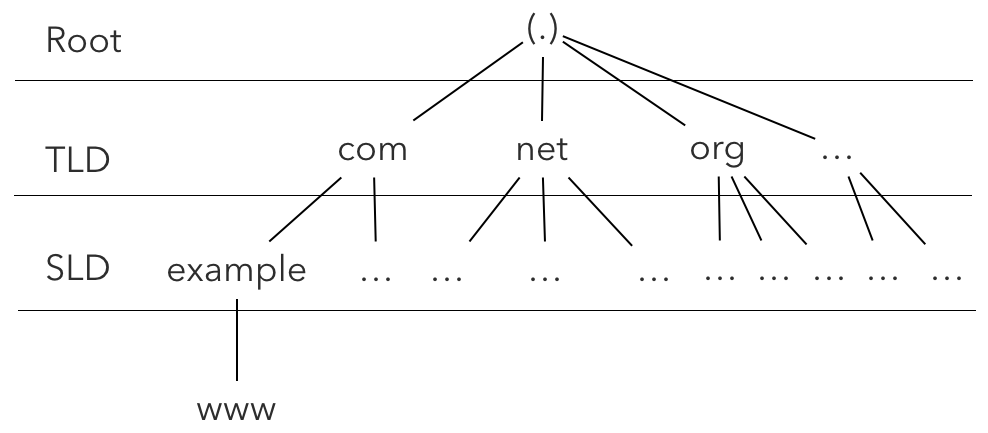
\includegraphics[width=12.0cm]{figure/dns-architecture.png}
 \caption{ドメインにおけるゾーンごとの名前空間}
 \label{fig:dns-architecture}
\end{figure}

\textbf{アーキテクチャ}\\
DNSは,クライアント・サーバアーキテクチャで構成され,機能に基づき3つのサービスに分類することができる.
\begin{itemize}
 \item スタブリゾルバ
 \vspace{-3mm}
 \item フルサービスリゾルバ
 \vspace{-3mm}
 \item 権威サーバ
\end{itemize}

スタブリゾルバは,名前解決の問い合わせるを依頼するクライアントノードである.
フルサービスリゾルバ(キャッシュサーバ・リカーシブサーバとも呼称される)は,スタブリゾルバに代わって,リソースレコードを保持する権威サーバに問い合わせるクライアントノードである.
名前解決をする際には,ルートから順にTLD,SLDという具合に権威サーバに再帰的に問い合わせることで,最終的に目的のドメイン名に関するリソースレコード情報を取得する.
この時,はじめのルート権威サーバのアドレスは``root.hints"と呼ばれるファイルに基づいて問い合わせるが,それより下位のドメインについては,上位の権威サーバが次の権威サーバのアドレスを応答することで名前解決のチェーンを繋げている.
すなわち,ルート権威サーバがTLDの権威サーバのアドレスを応答し,TLDの権威サーバがSLDの権威サーバーのアドレスを応答していく具合である.
権威サーバは,リソースレコードを保持するサーバノードであり,フルサービスリゾルバからの問い合わせ依頼に応答する.

\begin{figure}[h]
 \centering
 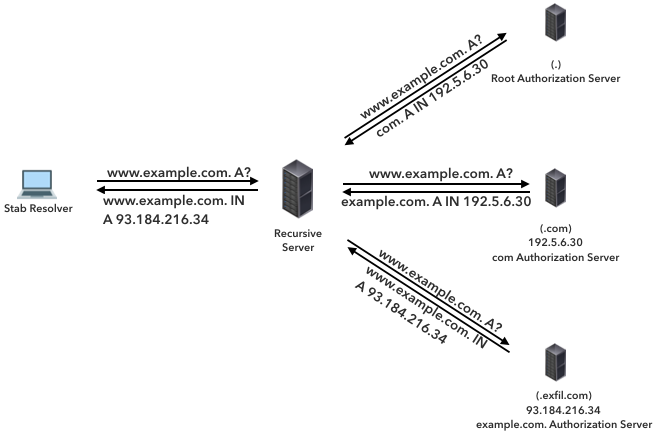
\includegraphics[width=12.0cm]{figure/dns-name-resolution.png}
 \caption{DNSによる名前解決}
 \label{fig:dns-name-resolution}
\end{figure}

\subsubsection{名前解決の仕組み}
\label{sec:dns-mechanism}
いま,クライアントから``www.example.com"のIPv4アドレスについて問い合わせられた場合を考える.
クライアントとなるスタブリゾルバは,スタブリゾルバと同一セグメント内のフルサービスリゾルバもしくは,ネットワークセグメントに依らないパブリックなフルサービスリゾルバ(オープンリゾルバ,パブリックリゾルバとも呼称される)に問い合わせる.
フルサービスリゾルバは,その名前解決クエリが過去に解決したものでないかキャッシュデータを確認する.
キャッシュにヒットした場合にはキャッシュの情報をクライアントに応答され,ヒットしなかった場合には,root.hintsファイルを参照しルート権威サーバにリクエストパケットを転送する.
クエリ(問い合わせ)を受け取ったルート権威サーバは,``com"ドメインを委譲した権威サーバのアドレスを応答する.
次に,フルサービスリゾルバは,``com"の権威サーバに対し同じクエリを転送する.
``com"の権威サーバは,``example.com"ドメインを委譲した権威サーバのアドレスを応答する.
フルリゾルバは,``example.com"の権威サーバに同じクエリを転送する.
``example.com"の権威サーバは,保持するゾーンファイルからクエリされたドメインのリソースレコードについて探索し,探索の結果としてレコード情報をフルサービスリゾルバに応答する.
フルサービスリゾルバは,権威サーバから応答された情報をスタブリゾルバに転送することで,問い合わせられた名前は解決される.
DNSによる名前解決の一連の動作を図~\ref{fig:dns-name-resolution}で示す.

%TLDごとに登録するプロセスや必要書類,金額は異なり,上位

\subsubsection{ドメイン名とリソースレコード}
\begin{figure}[h]
 \centering
 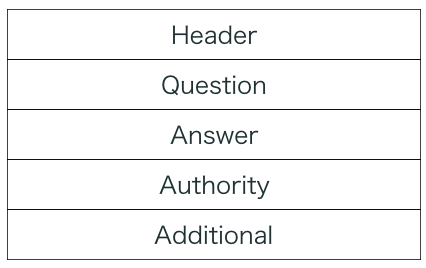
\includegraphics[scale=0.7]{figure/dns-format.png}
 \caption{DNSのパケット構造}
 \label{fig:dns-format}
\end{figure}

ドメイン名は,ルートから伸びる逆ツリー構造をドメインを表すラベルをドットで区切り表記する.
すなわち,ドメイン名は``label3.label2.label1."という具合にラベルを連結したものである.
右端のドットがルートを表現するが,全てのドメインがルートを頂点としているため,一般にルートを表す右端のドットは省略される.
図~\ref{fig:dns-format}は,DNSのパケット構造を表す.

\begin{figure}[h]
 \centering
 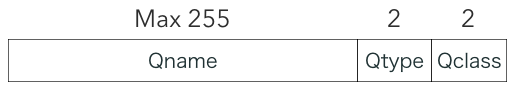
\includegraphics[scale=0.6]{figure/dns-answer.png}
 \caption{DNSのパケットのAnswerセクション}
 \label{fig:dns-answer}
\end{figure}

解決したいドメイン名は,図~\ref{fig:dns-answer}におけるQnameフィールドである.
各フィールドはサイズが決まっており,Qnameフィールドが最大長255バイト,リソースレコードのタイプを表すQtypeフィールドとクエリクラスを表すQclassフィールドがそれぞれ2バイトとなっている.

\begin{eqnarray}
 (LablD).(LabelC).(LabelB).(LabelA). \label{eq:domain-name} \\
 (Length) + (LabelD) + ... + (length) + (LableB) + (length) + (LabelA) + 0 \label{eq:label-name} \\ 
 1 + (Max 63) + ... + 1 + (Max 63) + 1 + (Max 63) + 1 = (Max 255) \label{eq:length-label-domain}
\end{eqnarray}

(\ref{eq:domain-name})は,複数のラベルで構成されたドメイン名の例である.
(\ref{eq:label-name})は,Questionヘッダーに注入される際のそのドメイン名を表すデータである.
Questionセクションでは,ドメイン名を表す際にドットは省略され,ラベルの長さとラベル名,そしてドメイン名の終わりを意味する``0"で表現される.
(\ref{eq:length-label-domain})は,ラベルの長さとラベル名のサイズを表す.
ラベルの長さは,1バイトのサイズで表現され,ラベル自体の最大長は63バイトである.
Questionセクションの最大長255バイトは,ラベルの長さとラベル,そしてドメイン終了を表す``0"を含めた長さである.
このため,最初のラベル長を表す1バイトとドメイン名の終了を意味する``0"を表すための1バイトを差し引いた253バイトが,実際のドメイン長の最大長である.

\begin{table}[htb]
 \centering
  \begin{tabular}{ccc}
    \toprule
		\textbf{タイプ} & \textbf{値} & \textbf{意味} \\
    \midrule
    A & 1 &  ホストのIPv4アドレス \\
    NS & 2 & 権威サーバ \\
    MF & 4 & メール転送サーバ \\
    CNAME & 5 & 別名 \\
    SOA & 6 & 権威ゾーンの開始 \\
    NULL & 10 & NULL(実験用) \\
    PTR & 12 & ドメイン名のポインター(逆引き) \\
    HINFO & 13 & ホスト情報 \\
    MINFO & 14 & メールボックスおよびメールリスト情報 \\
    MX & 15 & メール交換 \\
    TXT & 16 & 任意文字列 \\
    \bottomrule
  \end{tabular}
 \caption{主要リソースレコード一覧}
 \label{tab:resource-record}
\end{table}

ラベルには,数字とアルファベットおよびハイフン(``-")を使用することができ,ラベル中に大文字・小文字の区別はない.
他方で,アルファベットなどのASCII以外にも,国際化ドメイン名(IDN: Internationalized Domain Name)を使用すると日本語やアラビア語なども使用することができる.
IDNは,Punnycode~\cite{punnycode}\footnotetext{Punnycode: Unicode文字列を一意かつ可逆的にASCII文字列に変換する符号化方式}などのエンコーディング手法に基づき,DNSクエリする際にはASCIIコードに変換される.

ドメイン名に関連づけられる情報であるリソースレコードには複数のタイプが定義されており,目的ごとに使い分けられる.
例えば,Aというレコードタイプは,ドメイン名に対するIPv4アドレスを対応づけるために用いられる.
クライアントがあるドメイン名のIPv4アドレスが知りたいとき,スタブリゾルバは,ドメイン名とAのレコードタイプを指定することを希望のIPv4アドレスを取得することができる.
表~\ref{tab:resource-record}は,主要なリソースレコードである.


%リソースレコードのタイプごとの使用頻度を知りたい
% タイプごとの説明を充実させるのは,重要かもしれない


\subsection{DNSトンネリング}
\label{sec:dns-tunneling}
%DNSトンネリングが脅威となりうる点に関する説明
%Botnetなどに使用されることについて言及するべき
%概念
DNSトンネリングは,DNSをデータ転送のメディアとした秘匿通信手法の総称であり,転送元と転送先の方向性によって二つに分類することができる.
一つ目がDNS Exfiltrationと呼ばれる,スタブリゾルバから権威サーバ方向へのデータ転送手法であり,二つ目がDNS Infiltrationと呼ばれ,権威サーバからスタブリゾルバ方向へのデータを転送手法である.
%DNSトンネリングという手法は,ポートスキャンで知られるNmapのメーリングリストだとされている.
DNSトンネリングは,以下に示すDNSの特性に基づいた秘匿手法である.

\begin{itemize}
 \setlength{\itemsep}{0pt}
 \item 通常のインターネットの利活用において名前解決は必要な機能であるため,多くの組織でDNSのサービスポートが閉ざされることがない
 \item 名前解決のトラフィックはほとんどのサービスに先立って発生するため,クエリログが肥大化しやすく長期のログ保存が困難である
 \item パケットフォーマットの構造において,任意の文字列を注入できるフィールドを保持する
\end{itemize}

DNSトンネリングがデータ転送のキャリアとするフィールドは,クエリのQuestionセクションのQnameと,AnswerセクションのRdataである.
QuestionセクションのQnameフィールドを利用することで,スタブリゾルバから権威サーバ方向にデータを転送できる.
この方向の通信は,ビーコン通信やターゲットから取得した情報を外部に漏えいさせるといった攻撃の最終目的を達成するのに使われる.
また,AnswerセクションのRdataフィールドを利用することで,権威サーバからスタブリゾルバ方向にデータを転送することができる.
この方向の通信は,ターゲットネットワーク内のホストに潜伏したマルウェアなどへの命令コードを送信するのに使われる.
さらに,この二つのキャリアを利用することが双方向の通信路を確保できるため,C2通信を実施することも可能である.
%DNSトンネリング手法が脅威なのは,IDS・IPSなどの検知システムにフィルタリングされにくく,クエリ頻度を長期化させた場合解析を迂回することができる点である.

DNSトンネリングの手法は,ポートスキャンで知られるNmapのメーリングリストにて初めて一般に公開された(1998年)~\cite{nmap}.
その後,多くのDNSトンネリング実装~\cite{ozymandns, iodine, dnscat2, tcp-over-dns, dnscat, denise, dns-shell, dnsbotnet, dnscapy, dohtunnel, godoh, dohc2, magictunnelandroid, dns2tcp, tuns}が公開されながら,実際の攻撃に転化されるまでに至っている.


\subsubsection{スタブリゾルバから権威サーバ方向}
\label{sec:dns-exfiltration}

\begin{figure}[h]
 \centering
 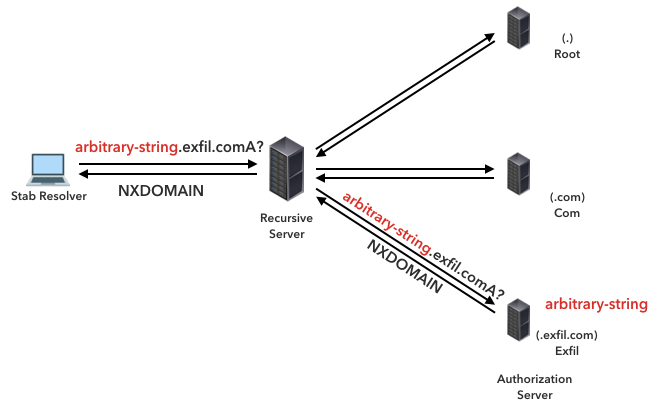
\includegraphics[width=12.0cm]{figure/dns-exfiltration.png}
 \caption{DNS Exfiltrationメソッドに基づいて,ドメイン名のラベル部に任意文字列(``arbitrary-string")が注入されたDNSクエリが,イントラネット内のスタブリゾルバからインターネット上の権威サーバ(``exfil.com")に転送される様子}
 \label{fig:dns-exfiltration}
\end{figure}


本項では,スタブリゾルバから権威サーバ方向にデータを転送する手法であるDNS Exfiltrationの詳細について説明する.

DNS Exfiltrationは,名前解決として問い合わせられるドメイン名が,そのドメインのゾーンを管理する権威サーバに転送される仕組みを利用した手法である.
DNSでは,ドメイン名に関連づけられるリソースレコードの情報は,そのドメインをゾーンとする権威サーバが保持しており,ルートから再帰的に問い合わせていくことでその権威サーバからの応答を受け取る.
このため,問い合わせられたドメイン名が実在しない場合でも,再帰問い合わせの仕組みに従って,そのドメイン名の最後の権威サーバまで転送されることになる.
権威サーバでは通常,クエリされたドメイン名の実在有無に寄らず,問い合わせられたクエリ情報をログとして管理する.
このような特性に踏まえてDNSを利用すると,DNSクエリのドメイン名のラベルに組織外ネットワークに転送したいの文字列を注入することで,組織外ネットワーク上に設置された権威サーバにそのデータを転送することができる.
これがDNS Exfiltrationの動作原理である.

このような仕組みで動作するDNS Exfiltrationを動作させるには,宛先となる権威サーバを用意する必要がありため,グローバルなドメインを取得することを前提としている.
第~\ref{sec:dns-mechanism}項で述べるように,ドメイン名の最大長は253バイトであり,その内ラベルの最大長は63バイトまでという制約がある.
そのため,DNS Exfiltration手法を用いてデータを転送する際には,TLDのラベルと宛先権威サーバのラベルもしくはSLDラベルと権威サーバのラベルを差し引いたサイズが実際に転送できる最大長となる.
また,任意の文字列をDNS Exfiltrationメソッドを用いて外部に転送するにあたり,転送キャリであるドメイン名における文字列制約を満たすように転送したいデータに前処理を施す必要がある.
ドメイン名に使用できる文字列は,第~\ref{sec:dns-mechanism}項で述べるように,``a"から``z"までのアルファベットと``0"から``9"までの数字と先頭以外のハイフン``-"記号である.
この文字列制約については,転送したいデータをバイナリデータに変換し,そのバイナリデータをラベルとして印字可能なASCIIコードに変換することでその制約を満たすことができる.
この前処理について,既存のDNSトンネリング実装の多くがBase Encoding~\cite{rfc4648}を用いている.
%使用するエンコーディング手法によって,データの圧縮率は異なる.
この処理によって,転送データがバイナリデータである際にも転送効率上げたり,ラベルの文字列制約を満たさないデータも転送することができる.
また,メッセージの意味抽出を困難にするためのトリックとして用いられる.

いま,DNS Exfiltrationを用いて,あるイントラネット内のホストからイントラネット外のホストにデータを転送することを考える.
転送される宛先となるイントラネット外のホストには,``exfil.com"より下位の全ての名前空間をゾーンとする権威サーバ(``exfil.com")を指定する.
転送したい文字列にエンコーディング前処理を施した後,``<用意した文字列>.exfil.com"という具合に文字列をラベルとして含めることで,ドメイン名が用意できる.
適当なリソースレコードタイプを指定し,DNSクエリとして転送すると,その権威サーバにはログとして,文字列を含んだドメイン名を取得する.
最後に,受け取ったサーバサイドは,前処理と逆のデコード処理を施すことで,オリジナルのデータを取得できる.
以上のように再帰問い合わせとラベルという転送キャリア,エンコーディング処理を組み合わせることで,イントラネット内のホストから外部ネットワークに任意の情報を転送することができる.
これが,DNS Exfiltrationの動作メカニズムである.
図~\ref{fig:dns-exfiltration}に,DNS Exfiltrationのメカニズムを図解した様子である.

%具体的な脅威モデル
%検知バイパス手法 : スループット(パフォーマンス)を下げることによる秘匿性,一般的なホスト名を使った対応表

%1998年4月,DNSトンネリングの手法は,NmapのBugtraqメーリングリストにて初めて公になったとされている\cite{bugtraq}.

\subsubsection{権威サーバからスタブリゾルバ方向}
\label{sec:dns-infiltration}

\begin{figure}[h]
 \centering
 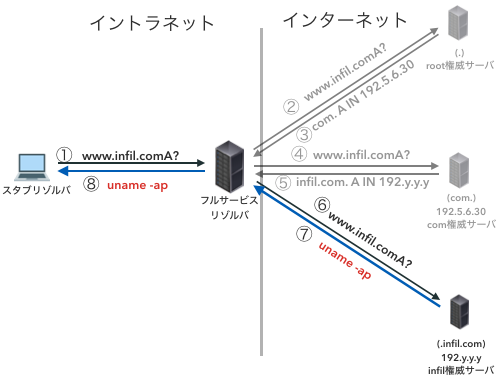
\includegraphics[width=10.0cm]{figure/dns-infiltration.png}
 \caption{TXTレコードに登録された情報について,DNSクエリで問い合わせることで権威サーバから命令情報を取得している様子}
 \label{fig:dns-infiltration}
\end{figure}

本項では,権威サーバからスタブリゾルバ方向にデータを転送する手法であるDNS Infiltrationの詳細について説明する.

DNS Infiltrationは,DNSにおける幾つかのリソースレコードが任意の文字列を記述できる設計を利用したデータ転送手法である.
ドメイン名に関連づけられた情報を管理・提供する権威サーバは,ゾーンファイルに関連づけたい情報を記述する.
リソースレコードには,レコード情報を検証する機構が備わっていないため,任意の文字列を登録することができる.
特に,記法が決まっていないTXTタイプやNULLタイプなどもあり,DNS Infiltrationではこのようなレコードタイプに転送したいデータを登録しておく.
このようにして登録されたレコード情報について,名前解決問い合わせすることによって,インターネット(権威サーバ)からイントラネット(スタブリゾルバ)にデータを転送することができる.
DNS Infiltrationとして利用され得るレコードタイプについて,これまでのトンネリング実装で使用されたものに基づいてまとめたのが,表~\ref{tab:infil-rtype}である.
%zonefileを説明
%Infilとして使用される脅威のあるRtypeを列挙

\begin{table}[h]
 \centering
  \begin{tabular}{lrll}
    \toprule
		\textbf{タイプ} & \textbf{\begin{tabular}{c}最大サイズ\\(byte)\end{tabular}} & \textbf{説明} & 実装\\
    \midrule
		A & 4 & \ ホストのIPv4アドレス &\\ \hline
		NS & 4 & \ 権威サーバ & \ \cite{dnscat2}\\ \hline
    %MF & 4 & メール転送サーバ \\
		CNAME & 253 & \ 別名 & \ \cite{iodine},\cite{dnscat2}, \cite{dnscapy}, \cite{tuns}\\ \hline
		%SOA & 253 & 権威ゾーンの開始 & \\
		NULL & 255 & \ NULL(実験用) & \ \cite{iodine}\\ \hline
		PTR & 4 & \begin{tabular}{l}ドメイン名のポインター\\(逆引き)\end{tabular} & \\ \hline
    %HINFO & 13 & ホスト情報 \\
    %MINFO & 14 & メールボックスおよびメールリスト情報 \\
		MX & 253 & \ メール交換 & \ \cite{iodine},\cite{dnscat2}\\ \hline
		TXT & 255 & \ 任意文字列 & \begin{tabular}{l}\cite{iodine},\cite{dnscat2}, \cite{denise}, \cite{dns-shell},\\ \cite{dnscapy}, \cite{dohtunnel}, \cite{dohc2}\end{tabular}\\ \hline
		AAAA & 32 & \ ホストのIPv6アドレス & \\ \hline
		SRV & 180 & \begin{tabular}{l}ドメイン名に対する\\サービスの場所\end{tabular} & \ \cite{iodine}\\ \hline
		 DNSKEY & 40 & \ DNSSECのための公開鍵 & \ \cite{dns2tcp}\\
    %TLSA & 52 & \\
    \bottomrule
  \end{tabular}
 \caption{DNS Infiltrationのメソッドとして使用することができるレコードタイプの一覧}
 \label{tab:infil-rtype}
\end{table}

NS・CNAME・MXレコードでは,DNS Exfiltrationと同じ要領でドメイン名のラベルに転送したい文字列を注入できる.
また,NULL・TXT・SRV・DNSKEYを用いる場合には,レコード構文の指定がないため文字列をそのまま注入できる.
最後に,A・AAAA・PTRレコードを用いる場合には,転送したい文字列を数字に変換させた後に,ドット(.)区切りもしくはコロン(:)区切りで注入できる.

いま,TXTレコードタイプを用いてDNS Infiltrationすることを考える.

(\ref{eq:infil-txt})で示すように,権威サーバは,転送したい文字列をゾーンファイルのTXTレコードとして登録する.
\begin{eqnarray}
 www.exfil.com \qquad IN \quad TXT \quad ``rm -rf \ /"
 \label{eq:infil-txt}
\end{eqnarray}
次に,スタブリゾルバは,``www.exfil.com"の``TXT"レコードタイプを通常通り問い合わせる.
後は,再帰問い合わせの仕組みに基づいて,そのDNSクエリは``exfil.com"まで転送され,ゾーンファイルの``TXT"レコードタイプの値がフルサービスリゾルバを経由したのち,スタブリゾルバまで応答される.
DNS Infiltrationの流入通信を図解した様子が,図~\ref{fig:dns-infiltration}である.
このようにして,DNS Infiltrationでは,正規の名前解決の方法を用いて,インターネットから組織内へとデータを取得することができる.

% Null タイプは,厳密に定義されておらず,実験用としか表現されていない.しかし,全体のタイプのうち,20%を示す程度に頻繁に使用されるタイプのである.

\subsection{検知に基づく既存対策手法}
本節では,DNSトンネリングに対するこれまでの対策手法について説明する.
% 検知に基づく手法の現在までの程度を淡々と示す.
\subsubsection{特徴量}
本項では,DNSトンネリングメソッドを使用した際に出現する傾向のある特徴量について説明する.

%長さ
一つ目が,表~\ref{tab:feature-tunnel}で示すように,Qnameフィールドのドメイン名の長さとパケットサイズである.
例えば,DNS Exfiltrationにおいて,一回あたりのデータ転送量を増加させる場合,Qnameフィールドのドメイン長もそれに比例して長くなり,結果としてパケットサイズも増加するという具合である.
DNS Infiltrationにおいても同様で,一回あたりのデータ転送量を増加させる場合,Rdataフィールド内のデータ量も大きくなり,応答パケットのサイズが増加する.
このことから,ドメイン名の長さとパケットサイズはDNSトンネリングの特徴といえる.

\begin{table}[th]
 \caption{正規DNSクエリとDNSトンネリングにおけるドメイン名の違い}
 \centering
  \begin{tabular}{l|l}
    \toprule
		\multicolumn{1}{c}{\textbf{種類}} & \multicolumn{1}{c}{\textbf{ドメイン名}} \\
    \midrule
    正規 &  www.example.com \\ \hline
    トンネリング & arbitrary-long-text-utill-it-reaches-253byte.example.com\\
    \bottomrule
  \end{tabular}
 \label{tab:feature-tunnel}
\end{table}


%同一ドメインあたりのクエリ頻度
二つ目が,同一ドメインに対するトラフィック頻度についてである.
例えば,転送したいデータが大きい場合,一回につき転送できるデータ量には限界があるため,複数のパケットに分割することによって転送する手法が考えられる.
このため,同一ドメインに対して,ラベルの異なるDNSクエリが多数発生することとなる.
同様にして,大きなデータサイズの情報をクライアントに転送する際には,複数のトラフィックが発生することになる.
以上のことから,特定の時間あたりで同一ドメインに対して,トラフィックが急激に増加するものをDNSトンネリングと判断できる可能性があることがわかる.

%レコードタイプ
三つ目は,リソースレコードのタイプについてである.
この特徴は,DNS Infiltrationメソッドを使用する際に出現する.
第~\ref{sec:dns-infiltration}で述べるように,DNS Infiltrationでは,リソースレコードをデータ転送のキャリアとして利用する.
しかし,通常のインターネットの利活用において使用されるリソースレコードのタイプには,偏りが存在することが知られている.
Tatangら~\cite{tatang}が,2017年7月30日から9月1日までの期間にて,取得した

\begin{table}[h]
 \caption[リソースレコードの分布]{2017年7月から8月までのDNSトラフィックデータセットにおけるリソースレコードのタイプ分布}
 \centering
  \begin{tabular}{lrr}
    \toprule
    \textbf{タイプ} & \textbf{パケット数} & \textbf{割合(\%)}\\
    \midrule
    A & 1,121,025,638 & 54.90\\
    AAAA & 197,388,865 & 9.67\\
    MX & 682,948 & 00.3\\
    NS & 7,662,147 & 0.38 \\
    CNAME & 156,708,021 & 7.68 \\
    TXT & 41,593,164 & 2.04 \\
    NULL & 432,232,574 & 21.17 \\
    Other & 84,371,709 & 4.13 \\
    \bottomrule
  \end{tabular}
 \label{tab:infil-rtype}
\end{table}


による調査では,表~\ref{tab:distribution-rr}で示す通り


%具体的な頻度の図を引用しよう
%Qnameにおける文字列分布とエントロピー
最後に,Bornら~\cite{born}およびChengら~\cite{cheng}によって明らかにされた文字列の分布とエントロピーの特徴がある.
著者らは,ドメイン名に出現する文字の出現頻度に着目することで,DNSトンネリングメソッドをしようした場合にランダムなドメイン名となる傾向にあることを明らかにした.
著者らは,正規のドメイン名と自然言語である英語,およびDNSトンネリングにおけるドメイン名に文字の出現頻度をそれぞれ評価した.
結果として,正規のドメイン名が英語の自然言語における文字の出現頻度に高い相関関係を示すのに対して,DNSトンネリングにおけるドメイン名と英語には相関がないことから,DNSトンネリングメソッドをしようした場合,ランダムな文字列で構成されるドメイン名となる傾向であることを示している.

これは,本来DNSでは,人が認知しやすくするためにドメイン名を用いるため,正規のドメイン名を作成するとき自然言語に近いラベルを作成する傾向にあることが推測できる.
これに対して,DNSトンネリングメソッドを使った場合には,文字列を注入する際にラベルの文字列制約を満たすためにバイナリおよびASCIIコードに変換する必要があり,このためラベルに意味を持たせる


\subsubsection{閾値推定}
\subsubsection{機械学習に基づくモデル}
%\subsubsection{パターンマッチング}
%\subsubsection{課題 : Low ThroughputなTunnelingに対する検知手法}
DNSトンネリングメソッドを使用した時のDNSクエリは,で述べるような特性が出現する.
この性質に基づき,これまでに多数の検知手法が提案されてきた.

\subsubsection{検知迂回手法}
%パフォーマンスを下げる手法(Low Latency)
%DNSエイリアスに対応づける手法
% 慣習的に命名されるラベル(Naming Convention)に意味を持たせることによって,例えば1byteの情報を持たせること
%特別Alexaなどの人気ラベルを調査しなくてもいいのかもしれない
